\documentclass[11pt]{article}
\usepackage[utf8]{inputenc}
\usepackage[T1]{fontenc}
\usepackage{amsmath}
\usepackage{amssymb}
\usepackage{textcomp}


% Let pdflatex render the few raw unicode math/greek glyphs that creep into the
% prose, instead of crashing the build. Add new ones here as needed.
\DeclareUnicodeCharacter{2248}{\ensuremath{\approx}}   % ≈
\DeclareUnicodeCharacter{00B1}{\ensuremath{\pm}}       % ±
\DeclareUnicodeCharacter{00B2}{\ensuremath{^2}}        % ²
\DeclareUnicodeCharacter{03B1}{\ensuremath{\alpha}}    % α
\DeclareUnicodeCharacter{03B2}{\ensuremath{\beta}}     % β
\DeclareUnicodeCharacter{03B4}{\ensuremath{\delta}}    % δ
\DeclareUnicodeCharacter{03BA}{\ensuremath{\kappa}}    % κ
\DeclareUnicodeCharacter{03C3}{\ensuremath{\sigma}}    % σ
\DeclareUnicodeCharacter{03C6}{\ensuremath{\varphi}}   % φ
\DeclareUnicodeCharacter{03B8}{\ensuremath{\theta}}    % θ
\DeclareUnicodeCharacter{0394}{\ensuremath{\Delta}}    % Δ
\DeclareUnicodeCharacter{2264}{\ensuremath{\leq}}      % ≤
\DeclareUnicodeCharacter{2265}{\ensuremath{\geq}}      % ≥
\DeclareUnicodeCharacter{00D7}{\ensuremath{\times}}    % ×
\DeclareUnicodeCharacter{2192}{\ensuremath{\rightarrow}} % →
\usepackage[margin=1in]{geometry}
\usepackage{xcolor}
\usepackage{graphicx}
\usepackage{float}
\usepackage{caption}
\usepackage{hyperref}

\usepackage{xspace}
\newcommand{\clockref}{\textit{Clock-Reference}\xspace}
\newcommand{\extset}{\textit{Extended-Set}\xspace}
\newcommand{\drososet}{\textit{Drosophila-Set}\xspace}
\newcommand{\sigmaU}{\ensuremath{\sigma_u}\xspace}
\newcommand{\scritmo}{\textit{scRitmo}\xspace}
\newcommand{\sigmabio}{$\sigma_\text{bio}$\xspace}
\newcommand{\sigmatech}{$\sigma_\text{technical}$\xspace}
\newcommand{\sigmadata}{$\sigma_\text{data}$\xspace}

% --- Math notation for the variance decomposition (R2.1 to R2.3) ---------
% Same symbols as the Obsidian notes (variance_decomposition_two_shells.md).
% Group b = one replicate at one ZT. theta = true phase, \that = inferred phase.
\DeclareMathOperator{\Var}{Var}
\newcommand{\E}{\mathbb{E}}
\newcommand{\that}{\hat\theta}
\newcommand{\ii}{\mathrm{i}}
\newcommand{\sbio}{\ensuremath{\sigma_{\text{bio}}}\xspace}          % math safe \sigmabio
\newcommand{\sbiob}{\ensuremath{\sigma_{\text{bio},b}}\xspace}       % biological spread of group b
\newcommand{\Tb}{T_b}                                                % exact technical term of group b
\newcommand{\Bb}{B_b}                                                % exact biological term of group b
\newcommand{\Vb}{V_b}                                                % observed variance of inferred phases, group b
\newcommand{\pb}{p_b}                                                % distribution of true phases in group b
\newcommand{\mub}{\mu_b}                                             % mean true phase of group b
\newcommand{\fc}{f_{\circ}}   % technical variance on the circle, -2 ln r
\newcommand{\Rbar}{\bar R_b}                                         % mean resultant length of inferred phases, group b

% --- Figure cross-references ---------------------------------------------
% Rebuttal's own figures: \rebfig{label} -> "Fig. Reb N";
% optional first arg is the panel, e.g. \rebfig[A]{fig:decomposition} -> "Fig. Reb 2A".
% The \ref keeps numbering automatic, so reordering figures never breaks the text.
\newcommand{\rebfig}[2][]{Fig.~Reb~\ref{#2}#1}
% Main-paper figures: their numbers live in the paper repo (no label here), so
% \mainfig{2C} -> "Fig. 2C of the main text", \mainfig{S1E} -> "Fig. S1E of the main text".
\newcommand{\mainfig}[1]{Fig.~#1 of the main text}
% Main-paper equations not reproduced in the rebuttal: \maineq{3} -> "Eq. 3 of the main text".
\newcommand{\maineq}[1]{Eq.~#1 of the main text}


% --- Formatting helpers --------------------------------------------------
% Reviewer comment, rendered in italics
\newcommand{\reviewer}[1]{{\itshape #1}\par\medskip}
% Our response label
\newcommand{\response}{\par\noindent\textbf{Response.}\ }
% Sub-heading inside a response: small caps, not bold, on its own line.
% Used with \paragraph{...} at the start of each block of a long answer.
% A full empty line (\baselineskip) is left before every heading, on purpose.
\renewcommand{\paragraph}[1]{%
  \par\vspace{\baselineskip}
  \noindent\textsc{\small #1}\par\nopagebreak 
}
% Rebuttal figures are labelled "Figure Reb N"
\renewcommand{\figurename}{Figure Reb}

\title{Response to Reviewers, Round 2\\[4pt]
\large Inferring circadian phases and quantifying biological desynchrony
across single-cell transcriptomes}
\author{Salati \textit{et al.}}
\date{September 2026}

\begin{document}

\maketitle

\noindent We thank both reviewers for their second round of comments.
Below we reproduce each comment (in \textit{italics}) followed by our response.

\medskip
\noindent\textit{A note on numbering.} % TODO: fill in once the revised numbering is fixed.
Figure, panel and equation references in our responses are to the revised manuscript
unless stated otherwise. References of the form Fig.~Reb~N point to figures of this document or of the first round response.

\bigskip
\noindent\textbf{Summary of main changes.}

\begin{itemize}
\item % TODO
\end{itemize}

\bigskip
\hrule
\bigskip

% Figure commands are defined in figures.tex, then placed inline next to the relevant reply.
% !TeX root = main.tex
% =========================================================================
% REBUTTAL FIGURES (round 2): one \newcommand per figure, typeset with [H]
% and the caption placed outside the float with \captionof{figure}{...},
% same pattern as ../rebuttal/figures.tex. Example:
%
% \newcommand{\figExample}{%
% \begin{figure}[H]
%   \centering
%   \includegraphics[width=\linewidth,height=0.95\textheight,keepaspectratio]{figures/FIGURE_example.pdf}
% \end{figure}
%
% \captionof{figure}{\textbf{Title.} \textbf{(A)} ...}
% \label{fig:example}
% }
% =========================================================================

% ------------------------------------------------------------------ R2.3b
\newcommand{\figRampFish}{%
\begin{figure}[H]
  \centering
  \begin{minipage}{\linewidth}
  \centering
  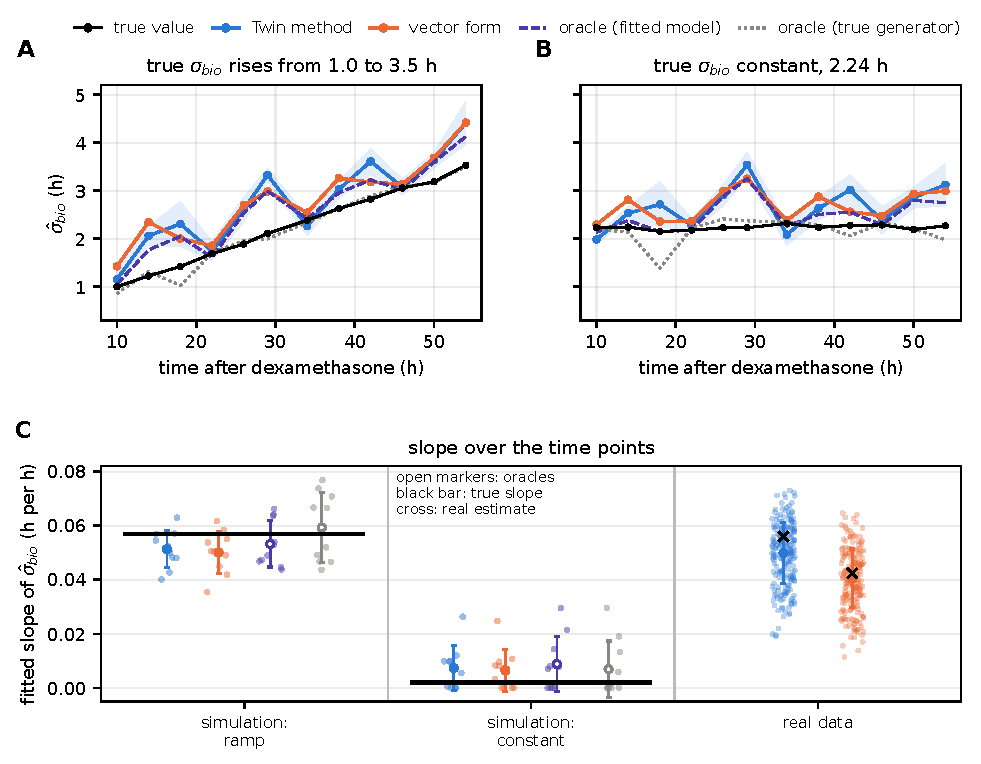
\includegraphics[width=0.9\linewidth,height=0.47\textheight,keepaspectratio]{figures/FIGURE_ramp_fish.pdf}

  {\footnotesize
  \captionof{figure}{\textbf{A simulated copy of the SABER-FISH experiment, with a known $\sigma_{\text{bio}}$ at each time point, next to the real data.}
  \textbf{(A, B)} The estimates follow a rising true $\sigma_{\text{bio}}$ but sit above it. Simulation from the fitted model of the real data (4 genes), with the 12 time points and the numbers of cells of the real experiment and the cell areas of the real cells of each time point as library sizes. The model was fitted again on each of the 10 simulated datasets, and the estimates were made with the same settings as for the real data. Estimated $\sigma_{\text{bio}}$ at each time point when the true value rises from 1.0 to 3.5 h (A) and when it is constant at 2.24 h (B). Black: true value, the circular standard deviation of the true phases of the simulated cells of that time point, so it varies a little around the design value. Blue and orange: Twin method and vector form, mean over the replicates. Blue band: standard deviation of the Twin method over the replicates (the band of the vector form is similar). Dashed purple: oracle with the fitted model, which knows the true phase of every cell and simulates the time point again with the fitted model. Dotted grey: the same oracle with the model that generated the data. The time point at 18 h has the fewest cells (116).
  \textbf{(C)} The slope is recovered in simulation, and it is smaller and less certain in the real data. Slope of the line fitted to the estimates of the 11 time points after the first one, as for the real data (the slope is not allowed to be negative). Same colors as in A. The two oracles have open markers (fitted model in purple, true generator in grey). Black bar: slope of the same line fitted to the true values. Small dots: the 10 replicates for the simulations, and 50 bootstrap draws over the cells for the real data (the model is not fitted again in the bootstrap, so the spread of the dots is smaller than it would be with a new fit). Large markers: mean and standard deviation of the dots. Cross: slope of the real estimates without the bootstrap.
  \textbf{(D)} The real estimates scatter more than the simulated ones. Real data, 116 to 362 cells per time point. Twin method and vector form with the 95\% bootstrap interval over the cells (points are shifted sideways by 0.5 h for legibility). At 18 h the observed spread is smaller than the technical spread, and the Twin estimate is set to zero.}
  \label{fig:ramp_fish}
  }
  \end{minipage}
\end{figure}
}

% ------------------------------------------------------------------ R2.3c
\newcommand{\figRampRnaseq}{%
\begin{figure}[H]
  \centering
  \begin{minipage}{\linewidth}
  \centering
  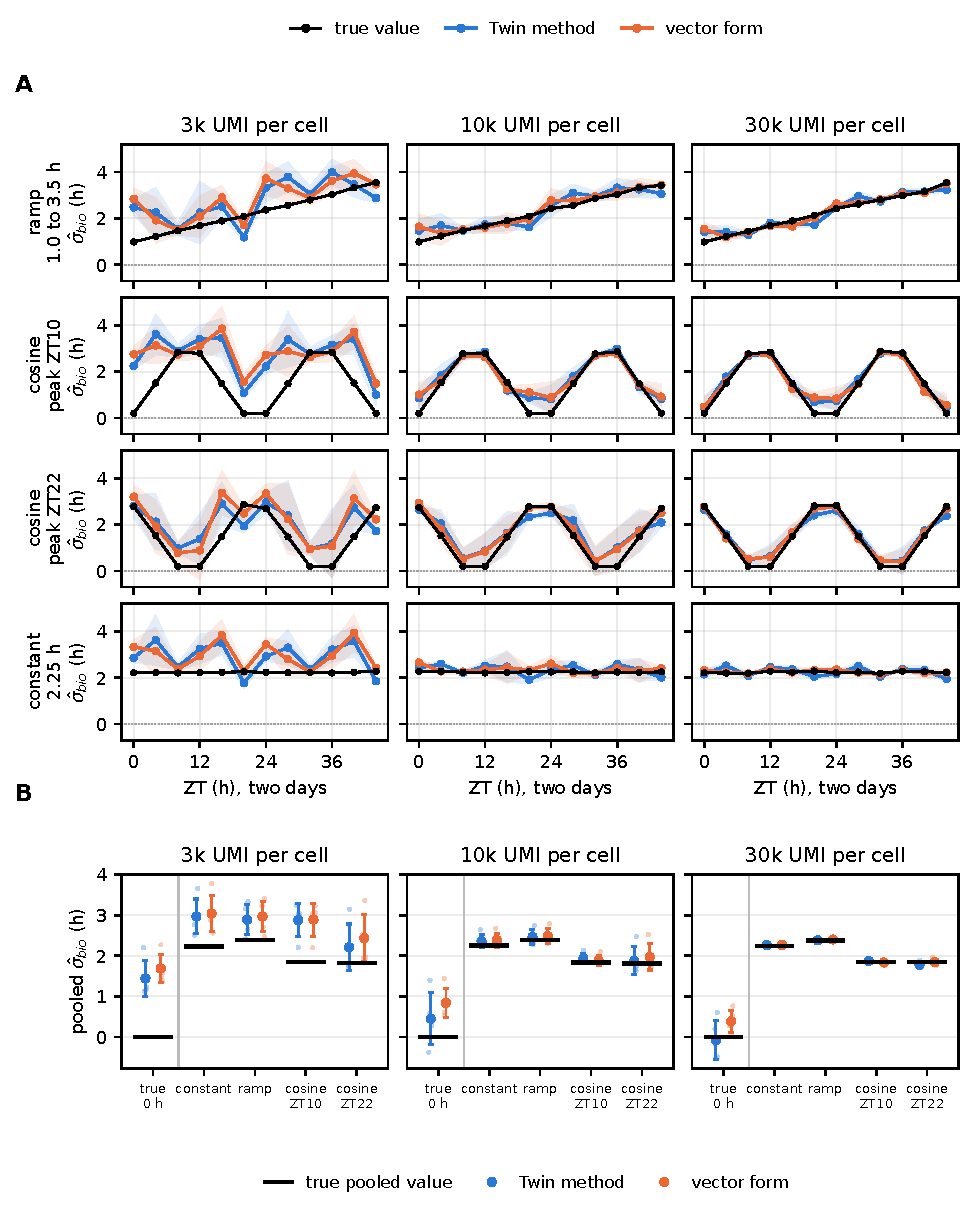
\includegraphics[width=\linewidth,height=0.72\textheight,keepaspectratio]{figures/FIGURE_ramp_rnaseq.pdf}

  {\small
  \captionof{figure}{\textbf{Simulations with a $\sigma_{\text{bio}}$ that changes across time points.}
  15 clock genes, 12 time points over two days, 500 cells per time point, 5 replicates per setting. Columns are the depths.
  \textbf{(A)} Estimated $\sigma_{\text{bio}}$ at each time point for four true profiles (rows). Black: true value. Lines: mean over the replicates. Bands: standard deviation over the replicates. The true cosine is sampled every 4 h (0.2 to 2.8 h) and repeats on the second day.
  \textbf{(B)} The single value over all time points (\maineq{16}) for the same profiles (cosine ZT10 and ZT22 are the two cosines of A) and for a control with a true $\sigma_{\text{bio}}$ of 0. Black bar: true value, the square root of the average of the true $\sigma_{\text{bio}}^2$ weighted by cell number. Large markers: mean and standard deviation over the replicates. Small dots: the 5 replicates.
  Twin method, vector form and oracle are defined in the text and in the response to R2.1.}
  \label{fig:ramp_rnaseq}
  }
  \end{minipage}
\end{figure}
}


% !TeX root = main.tex
\section*{Reviewer 1}

\bigskip

% ------------------------------------------------------------------ R1.1
\subsection*{R1.1 --- Phase at which the Twin-Dataset is constructed}

\reviewer{The phase at which the Twin-Dataset is constructed is never stated.
The Methods define the twin as a synthetic dataset reproducing the per-cell library sizes and sequencing depth of the data under study, in which every cell shares the same circadian phase, and Eq.~(15) then subtracts the resulting $\sigma_{\text{technical}}$ at ``the group's sequencing depth''.
Which phase the cells are placed at is not specified anywhere.
This is not a detail: the paper itself shows $\sigma_{\text{technical}}$ varying roughly two-fold around the cycle (Fig.~S1F), so the choice materially determines every reported $\sigma_{\text{bio}}$.
The response to my earlier point makes clear that the twin sits at the phase of the group it mirrors, and that this is precisely what protects the estimator from the phase-dependence concern I raised --- but a reader of the manuscript alone cannot reconstruct the central estimator.
One sentence in the Twin-Dataset paragraph would close this.}

\response

% ------------------------------------------------------------------ R1.2
\subsection*{R1.2 --- Derivation of the period spread}

\reviewer{Two problems in the derivation of the period spread.
The Methods state that fixed period heterogeneity and within-cycle stochastic phase fluctuations ``both produce a linearly growing cSTD, so they cannot be separated from a slope alone''.
Diffusive phase accumulation gives a variance linear in time and therefore a cSTD growing as the square root of time, whereas period heterogeneity gives a cSTD linear in time; the two have different time dependence.
The two references cited in that same sentence treat the contributions as distinguishable in principle. 
Please clarify.}

\response

% ------------------------------------------------------------------ R1.3
\subsection*{R1.3 --- Explanation of the phase dependence of $\sigma_{\text{technical}}$}

\reviewer{The explanation offered for the phase-dependence of $\sigma_{\text{technical}}$ does not match the periodicity reported.
The Results attribute the variation of $\sigma_{\text{technical}}$ across the cycle to ``the non-uniform distribution of peak phases across the rhythmic gene set'', which is a once-per-cycle effect.
Yet the SABER-FISH paragraph describes the modulation recovered in real data as 12h-periodic, and Fig.~S1F shows two maxima per cycle.
The dominant mechanism --- that a small phase error perturbs predicted expression in proportion to the local steepness of the cosine, which is flat at peak and at trough and steepest between them, giving two maxima per cycle --- is stated clearly in a footnote of the response and appears nowhere in the manuscript.
Uneven peak phases account only for the weaker once-per-cycle component.
Please move the correct explanation into the Results; it is two sentences, and it matters because this modulation is what makes the per-time-point $\sigma_{\text{bio}}$ values uneven, which the same paragraph goes on to discuss.}

\response

We thank the reviewer for catching this. The explanation in the Results was wrong. We have replaced it with the cosine steepness argument, which gives two maxima per cycle, and kept the uneven peak phases only as a weaker once per cycle component.

% ------------------------------------------------------------------ R1.4
\subsection*{R1.4 --- Supplementary tables and reproducibility}

\reviewer{Supplementary tables and reproducibility.
Tables S1, S2 and S3 are cited in the main text --- the Extended-Set gene parameters, the per-cell-type and per-time-point variance components, and the Drosophila-Set parameters respectively --- but are not present in the supplementary file supplied to me.
Please confirm they ship with the paper rather than only with the code repository; Table S2 in particular is the item I wanted to see and is the one a reader will want alongside Fig.~3J.
On the code itself, the position is now satisfactory in substance: both repositories are public and the preprocessed data are deposited.
I can think of one potentially useful addition, which is the lightweight cell bootstrap that the authors describe as running in seconds from the deposited per-cell phases.
I think this would be a very useful artefact in the repository if shipped as a standalone script.}

\response

\newpage
% !TeX root = main.tex
\section*{Reviewer 2}

\noindent\textit{Overall assessment.} The reviewer finds that several questions were answered satisfactorily but that the central methodological issues are not resolved: the statistical basis of the variance decomposition, the use of the SABER-FISH data given the averaging requirement, the weaker than stated uncertainty and $\sigma_u$ results, and the tone of the Abstract, Introduction and Discussion. The major points follow.

\bigskip

% ------------------------------------------------------------------ R2.1
\subsection*{R2.1 --- Conditioning variable of the decomposition within one ZT}

\reviewer{In response to my previous comment on the validity of their variance decomposition (R2.2 in the author's response), the authors argue that the conditioning variable $S$ in their Equation 13 (revised main text) is one replicate at one ZT time point and that the $\sigma_{\text{bio}}/\sigma_{\text{tech}}$ split is a ``further decomposition that lives entirely inside the within term''.
While this is OK, the author's decomposition purely within a ZT still must obey the law of total variance, since it is an identity that holds for any conditioning variable.
Therefore, if Eq.~14 is to be more than an analogy, it must itself be a total-variance decomposition within one single ZT timepoint with respect to some conditioning variable, and the authors need to precisely define what that variable is.
Otherwise, Eq.~14 appears quite ad hoc and it is impossible to interpret what the terms $\sigma_{\text{bio}}$ and $\sigma_{\text{tech}}$ are supposed to represent in a statistically rigorous framework.}

\response

% ------------------------------------------------------------------ R2.2
\subsection*{R2.2 --- Consistency with the law of total variance}

\reviewer{In the response R2.2, the authors go on to say that they ``never define $\sigma_{\text{tech}}$ as the within-term of a latent phase-cluster decomposition (an average over heterogeneous sub-populations)\dots\ so there is no averaging over sub-populations with differing variances to reconcile''.
Does this mean the author's procedure is not consistent with the Law of Total Variance, which must have an averaging procedure across sub-populations?
If so, when the authors say that ``At the level of individual time points the additivity is only approximate'', is the approximation coming partly from this departure from the Law of Total Variance?
These points should be more carefully discussed in the Main Text and Methods, since the current version provides little clarity or discussion on this important issue.}

\response

% ------------------------------------------------------------------ R2.3
\subsection*{R2.3 --- Aggregation across the cycle and the SABER-FISH analysis}

\reviewer{The revised Methods state that Eq.~14 ``becomes near-exact ($R^2 \approx 1$) only once variances are aggregated across populations that span the circadian cycle'', and draw from this the requirement that ``the data must cover most of the circadian cycle''.
In the response letter, the authors further comment that ``$\sigma_{\text{bio}}$ is a property of a population sampled across the cycle, not of an individual ZT''.
This is made explicit in Eq.~16 of the revised Main Text.
This then raises the following important questions which I do not currently understand:}

\subsubsection*{R2.3a}

\reviewer{How can this requirement be reconciled with the analysis of the SABER-FISH dataset, where each ZT is analyzed separately to get $\sigma_{\text{bio}}$ and $\sigma_{\text{tech}}$ estimates at each time point?
Given that this is the main dataset with direct experimental validation of the $\sigma_{\text{bio}}$ estimates, the analysis of this data and the limitations should be discussed more carefully.}

\response

\subsubsection*{R2.3b}

\reviewer{The aggregation requirements of the method as well as all the simulations the authors have performed (Fig.~Reb~3A and 3B) seem to require one ground truth $\sigma_{\text{bio}}$ for the entire population of cells across the different ZT time points.
However, this requirement seems directly in conflict with the SABER-FISH data, where $\sigma_{\text{bio}}$ increases with time post Dexamethasone synchronization.
Therefore, the authors need to give a clear justification for applying their method to this dataset.
If this is only a very approximate and empirical application of the method, the authors should accordingly tone down their claims of discovering increasing desynchrony and using this dataset as a strong validation of their method.}

\response

\subsubsection*{R2.3c}

\reviewer{All simulations in the manuscript appear to hold $\sigma_{\text{bio}}$ to one fixed number across ZT time points, which is why the aggregation procedure seems to work via some cancellations.
But if the $\sigma_{\text{bio}}$ per ZT changes, as is the case with the SABER-FISH data, wouldn't this fundamentally create issues in recovering the right $\sigma_{\text{bio}}$ estimates?
Aggregation here would probably recover some sort of average of the individual $\sigma_{\text{bio}}$'s, right?
Therefore in order to claim that scRitmo can extract meaningful increase of desynchrony over time, the authors should at least provide simulations where ground truth $\sigma_{\text{bio}}$ increases across ZTs within a single simulation.
This simulation should then be analyzed with scRitmo and the results benchmarked for accuracy.}

\response

\subsubsection*{R2.3d}

\reviewer{The equations for the aggregation and their corresponding description, both in the main text and response, are quite confusing because key quantities have been vaguely defined.
What exactly do the words ``condition'' and ``batch'' mean here?
What does the term $\sigma_b$ refer to in Eq.~16 of the revised main text?
None of these have been defined.}

\response

% ------------------------------------------------------------------ R2.4
\subsection*{R2.4 --- Aggregation with few ZT samples}

\reviewer{The authors also comment that the aggregation procedure creates a requirement of sufficient ZT samples across 24 hours.
In their simulations, they use 12 and 8 ZT samples, which is greater than the number of samples one would get from typical scRNA-seq datasets.
For example, the Auerbach et al paper which the authors analyze, had only 4 samples spaced 6 hours apart.
To better understand the limits of the aggregation procedure, the authors should demonstrate what happens in such limited datasets --- would accurate estimates of a population $\sigma_{\text{bio}}$ still be possible if there are just 4 samples?}

\response

% ------------------------------------------------------------------ R2.5
\subsection*{R2.5 --- Identical mRNA and protein oscillations in the FLASH-seq data}

\reviewer{In the application of the method to phase inference in asynchronized FLASH-seq data, I appreciate the new results presented and agree that they provide more evidence that biologically meaningful oscillations are being reconstructed.
However, I'm still puzzled by the fact that the mRNA and protein oscillations look identical, and not phase shifted at all.
The protein oscillation peak should be delayed by 2--4 hours as per a vast body of prior literature, which is not reflected in the results here.
How does one interpret this?
Does this suggest that in fact there are significant errors being made in phase assignment to the single cells?
If so, I would recommend discussing this in the Main Text and also toning down the statement ``The inferred phase accurately reconstructed the oscillation of both the endogenous (Rev-Erb$\alpha$) mRNA level and the Rev-Erb$\alpha$-Venus protein fluorescence'', since the meaning of ``accurately'' cannot really be quantitatively established in this setting.}

\response

% ------------------------------------------------------------------ R2.6
\subsection*{R2.6 --- Strength of the $\sigma_u$ claims}

\reviewer{In the main text the authors say ``Across all tissues, cells with higher posterior uncertainty $\sigma_u$ showed larger phase errors than cells with lower $\sigma_u$ (Fig.~S3C, E, F), consistent with the per-cell correlation between $\sigma_u$ and phase error''.
In the Discussion they say ``The posterior uncertainty $\sigma_u$ consistently predicts inference quality across simulations and diverse biological datasets, enabling principled quality control without external time labels.''
However, in the light of the new quantification of correlations between $\sigma_u$ and error (ranging from 0.08 to 0.35 in Fig.~Reb~10A), these statements seem quite disproportionate.
Even the highest of these correlation values at 0.35 is weak at best, and it is also unclear whether any of these would pass statistical tests of significance.
The authors should therefore report these magnitudes along with results from statistical tests in the Main text, and statements such as those above should be tempered accordingly.}

\response


% !TeX root = main.tex
% Appendix A: full description of the vector form (moved out of R2.1).
\newpage
\section*{Appendix A: the vector form}

This appendix describes the vector form estimator summarised in the response to R2.1. It uses the notation of R2.1: group $b$ of $n_b$ cells, true phase $\theta \sim \pb$, inferred phase $\that$, $\rho(\theta) = \E[e^{\ii\that} \mid \theta] = r(\theta)\, e^{\ii m(\theta)}$, and the approximations A1 to A3 of the Twin method. In scRitmo it is \texttt{estimate\_phase\_desynchrony(sigma\_tech\_method="deconvolution", deconv\_form="vector")}.

\paragraph{Starting point.}

Instead of correcting the approximations A1 to A3 one by one, we start from the exact identity of R2.1, Eq.~\eqref{eq:total-expectation}. Its left side is what the data give (estimated by the mean $\bar z_b$ of $e^{\ii\that_c}$ over the cells, with $\Rbar = |\bar z_b|$). On the right, $\rho(\theta)$ is the technical part, which depends only on the model and the library sizes, and $\pb$ is the biological part, whose width is \sbiob. The identity needs no expansion, and no assumption that $r$ is constant or $m(\theta) = \theta$.

\paragraph{Step 1, measure $\rho$ on a grid.}

At each of $N = 24$ phases $\phi_k = 2\pi(k-1)/N$ (1 h apart) we simulate Twin cells (1000 per run, 5 runs pooled, so $M = 5000$), infer their phases and take the mean unit vector $\hat\rho_k = \frac{1}{M}\sum e^{\ii\that}$ over the $M$ cells at $\phi_k$. This is a plain mean, so $\E[\hat\rho_k] = \rho(\phi_k)$. We keep the complex value, because its direction holds the bias.

\paragraph{Step 2, Fourier series.}

Since $\rho$ is periodic,
\begin{equation}
\rho(\theta) = \sum_{j=-J}^{J} c_j\, e^{\ii j\theta},
\qquad
c_j = \frac{1}{N}\sum_{k=1}^{N} \hat\rho_k\, e^{-\ii j\phi_k},
\qquad J = \lfloor N/2 \rfloor ,
\label{eq:fourier}
\end{equation}
where the term at $|j| = N/2$ is split in two halves, so that the series passes through every grid point.

\paragraph{Step 3, average over the biological distribution.}

We assume $\pb$ is a wrapped normal with center $\mub$ and width $\sigma$ in radians, where $\sigma$ is the trial value of $\sbiob$. For harmonic $j$ (period $24/j$ h),
\begin{equation}
\E_{\theta \sim \pb}\big[e^{\ii j\theta}\big] = \kappa_j(\sigma)\, e^{\ii j\mub},
\qquad
\kappa_j(\sigma) = e^{-j^2\sigma^2/2}.
\label{eq:kappa}
\end{equation}
The factor $\kappa_j$ lies between 0 and 1. A distribution that is wide compared with the period covers both the peak and the trough of the harmonic, and the average shrinks toward zero. Putting Eq.~\eqref{eq:fourier} into the right side of Eq.~\eqref{eq:total-expectation} gives the expected mean vector of a group,
\begin{equation}
\bar\rho_b(\sigma) = \E_{\theta \sim \pb}\big[\rho(\theta)\big] = \sum_{j=-J}^{J} c_j\, \kappa_{|j|}(\sigma)\, e^{\ii j\mub}.
\label{eq:rhobar}
\end{equation}
The grid gives all the $c_j$, so this is a known function of $\sigma$. Under the conditions where Eq.~14 is exact ($r$ constant, $m(\theta) = \theta$, and many cells), it reduces to Eq.~14.

\paragraph{Step 4, one equation with one unknown.}

For independent cells, $\E[\Rbar^2] = |\bar\rho_b|^2 + (1 - |\bar\rho_b|^2)/n_b$, where the second term comes from the $n_b$ products of a cell with itself. The estimate $\hat\sigma_{\text{bio},b}$ is the value of $\sigma$ that solves
\begin{equation}
|\bar\rho_b(\sigma)|^2 + \frac{1 - |\bar\rho_b(\sigma)|^2}{n_b} = \Rbar^2 .
\label{eq:vector-equation}
\end{equation}
Here $\Rbar$ and $n_b$ come from the data, the $c_j$ from the grid, and $\mub$ is the ZT of the group in the phase frame of the fitted model, so only $\sigma$ is unknown. We search $\sigma$ over $[0,\pi]$ and accept a root only if it is unique. If the data are tighter than the prediction at $\sigma = 0$ we set the estimate to zero. If no unique root exists, the group has no estimate. The estimand is $\sbiob$, the spread of $\theta$, and not $\Bb$.

\paragraph{What is removed.}

A1 disappears because Eq.~\eqref{eq:rhobar} averages $\rho$ over the whole distribution $\pb$. A2 disappears because $\rho$ contains the direction $m(\theta)$, so the bias is inside the prediction. The circular correction disappears because Eq.~\eqref{eq:vector-equation} compares mean vectors and does not add variances, and the finite $n_b$ term is included. A3 does not arise as a wrong placement, since $\mub$ is the known ZT. What remains is an offset between the phase origin of the fitted model and ZT 0 (0.2 to 0.55 h in our simulation), which affects both methods.

\paragraph{Assumptions that remain.}

The wrapped normal shape of $\pb$; a fitted model close to the data generating process; one library size distribution shared by all groups (otherwise we build one grid per group); independent cells; and a grid large enough that its own sampling noise is small next to that of the data. The case where $\sbiob$ changes from group to group, as in the SABER-FISH data, is tested in R2.3b and R2.3c.


\bigskip
\hrule
\bigskip

\bibliographystyle{unsrt}
\bibliography{ref}

\end{document}
